\documentclass[12pt]{standalone}
\usepackage{polyglossia}
\setdefaultlanguage{vietnamese}
\setotherlanguages{english}
\usepackage{fontspec}
\usepackage{
    amsmath, 
    amsfonts, 
    amssymb
}
\usepackage{unicode-math}
% \setmainfont{STIX Two Text}
% \setmathfont{STIX Two Math} 
\usepackage{xcolor}
\usepackage{tikz}

\begin{document}
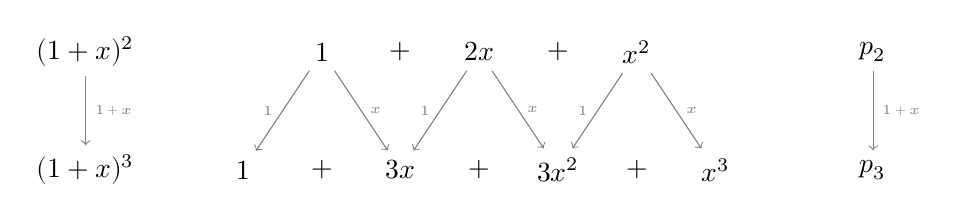
\begin{tikzpicture}%[level distance=1.5cm,sibling distance=2.5cm]
    % Dòng thứ hai
    \node (d21) at (-2, 10.5) {$1$};
    \node (d22) at (-1, 10.5) {$+$};
    \node (d23) at (0, 10.5) {$2x$};
    \node (d24) at (1, 10.5) {$+$};
    \node (d25) at (2, 10.5) {$x^2$};

    % Dòng thứ ba
    \node (d31) at (-3, 9) {$1$};
    \node (d32) at (-2, 9) {$+$};
    \node (d33) at (-1, 9) {$3x$};
    \node (d34) at (0, 9) {$+$};
    \node (d35) at (1, 9) {$3x^2$};
    \node (d36) at (2, 9) {$+$};
    \node (d37) at (3, 9) {$x^3$};
    
    % Các nhị thức tương ứng
    \node (d3l) at (-5,9) {$(1+x)^3$};
    \node (d2l) at (-5,10.5) {$(1+x)^2$};
    \node (d3r) at (5,9) {$p_3$};   
    \node (d2r) at (5,10.5) {$p_2$};   

    % Các đoạn thẳng
    \begin{scope}[every path/.style={color=gray}, every node/.style={color=gray,font=\tiny}]    
    \draw [->] (d21)--(d31) node[midway, left] {$1$};
    \draw [->] (d21)--(d33) node[midway, right] {$x$};
    \draw [->] (d23)--(d33) node[midway, left] {$1$};
    \draw [->] (d23)--(d35) node[midway, right] {$x$};
    \draw [->] (d25)--(d35) node[midway, left] {$1$};
    \draw [->] (d25)--(d37) node[midway, right] {$x$};
    
    \draw [->] (d2l)--(d3l) node[midway,right] {\(1+x\)};
    \draw [->] (d2r)--(d3r) node[midway,right] {\(1+x\)};

    \end{scope}
    
\end{tikzpicture}
\end{document}
